\documentclass[11pt,a4paper]{article}

\usepackage[margin=1in]{geometry}
\usepackage{amsmath,amssymb,amsthm}
\usepackage{graphicx}
\usepackage[hidelinks]{hyperref}
\usepackage{booktabs}
\usepackage{enumitem}
\usepackage{tikz}
\usepackage{xcolor}
\usepackage{titlesec}
\usepackage{microtype}
\usepackage{caption}
\usetikzlibrary{arrows.meta,positioning,fit,backgrounds,shapes.geometric,shadows}

\definecolor{abstrcol}{HTML}{2C5F8A}
\definecolor{numcol}{HTML}{D4850A}
\definecolor{boxbg}{HTML}{F5F5F5}

\titleformat{\section}{\Large\bfseries\color{abstrcol}}{\thesection}{1em}{}
\titleformat{\subsection}{\large\bfseries}{\thesubsection}{1em}{}

\newcommand{\abstr}[1]{\textcolor{abstrcol}{#1}}
\newcommand{\numr}[1]{\textcolor{numcol}{#1}}

\title{A Symbolic Substrate for Computational Materials Science:\\
       Design Notes, Decisions, and First-Demonstration Plan}
\author{G. Barbalinardo \\
        \small University of California, Davis}
\date{\today}

\begin{document}

\maketitle

\begin{abstract}
This document records the design of a typed substrate for computational materials science
workflows, together with the decisions and trade-offs that produced it. Workflows are directed
acyclic graphs of \emph{abstract physics states} connected by \emph{symbolic operations}, and
concrete numerical results are \emph{materializations}---typed projections of abstract states
into a discretization scheme. The substrate's abstract root is the \emph{Born--Oppenheimer
potential} of a material, expanded as a Taylor series in atomic displacements; force constants
of every order are derived states obtained by extracting derivatives of this root and truncating
the expansion at a chosen order. Every state carries a provenance chain that records the
operations along its path; every materialization carries a discretization scheme. Approximation
and discretization errors live in disjoint type universes and compose along graph edges; the
machinery for tracking error formulas symbolically and composing them across the graph is
designed but its full implementation is deferred to Phase 2. As a first demonstration, three
established lattice thermal-transport codes (kaldo, phono3py, ShengBTE) are reframed as distinct
materializations of a single abstract DAG, with cross-code reconciliation at canonical
intermediate states as the Phase 1 deliverable. Phase 1 stubs the upstream operations that
produce force constants from the potential---declaring the relevant abstract types and provenance
labels but not modeling them in detail---so that Phase 2 can elaborate the upstream without
restructuring the substrate. The document is intended as the working architectural reference for
the \texttt{openmaterials-ai} project; it covers each architectural decision, the alternatives
considered, and what we deferred.
\end{abstract}

\tableofcontents

\bigskip

\section{Background and Motivation}
\label{sec:motivation}

Modern computational materials science has many codes, many workflows, and many opinions about how
to compose them. Despite a generation of effort on workflow managers (\textsc{AiiDA}, \textsc{Atomate},
\textsc{FireWorks}, \textsc{Atomate2}, \textsc{Aflow}), one quality is still missing: a workflow
should expose, as typed and composable data, \emph{the physics it computes}.

Today the standard unit of shared meaning between codes is the \emph{input file}: an ordered
sequence of instructions that, together with a particular code's internal logic, produces an
output. This unit is opaque to two questions:

\begin{itemize}[leftmargin=2em]
  \item \textbf{Given a result, what physical assumptions and approximations does it embed?}
        An input file declares parameters but not their meaning. A k-mesh is just a triple of
        integers; the relationship between that mesh and the convergence of the integrated
        observable is not part of the file.
  \item \textbf{Given two results from two codes, where exactly do they diverge?} Identical force
        constants run through kaldo and through ShengBTE typically yield slightly different
        thermal conductivities. The difference is not localized to a particular operation, even
        though---in principle---it is the result of distinct computational choices at specific
        steps.
\end{itemize}

A previous attempt of ours, \texttt{MaterialsCodeGraph} (MCG), addressed parts of this gap by
treating each instruction in an input file as the atomic unit of a knowledge graph and tracking
inputs, parameters, and outputs at that level. MCG's tool-encapsulation principle (all tool
knowledge in YAML/Markdown configs, all code generic over tool) was the right design at that
level of abstraction. But the level of abstraction itself is too low: an instruction in an input
file is a syntactic unit, not a semantic one. It tells you what a code is told to do, not what
\emph{physics} the code thereby computes. Two codes that compute the phonon dispersion via
diagonalization of the dynamical matrix express that operation as different instructions; yet
they perform the same physics. A graph indexed by instructions sees them as two unrelated tasks.

\medskip

The substrate proposed here \emph{starts from the physics} and treats input files as derived
artifacts. The atomic unit is no longer an instruction; it is a \emph{symbolic operation} between
typed physics states. The states are the load-bearing entities: a state is what changes when an
operation is applied, and a workflow is the graph that records those state transitions. Concrete
numerical computation is then a separate, typed projection of the abstract workflow into a
discretization scheme.

This is a deliberate departure from the input-file paradigm. We argue below that it pays for the
extra abstraction with three concrete returns: cross-code reconciliation at canonical intermediate
states, derived (rather than empirical) error bounds on computed observables, and a clean
substrate for future formal verification.

\section{Architectural Principle: Two Worlds, One Bridge}
\label{sec:principle}

The single most important design decision is a strict separation between two type universes:

\begin{itemize}[leftmargin=2em]
  \item \abstr{\textbf{The abstract world}} holds typed physics states (Hamiltonians, dispersion
        relations, scattering rates, distribution functions, partition functions) and symbolic
        operations between them. Errors here are \emph{approximation errors}---the $O(\cdot)$
        terms introduced by truncating perturbation series, linearizing equations, or imposing
        physical assumptions such as the Born--Oppenheimer or harmonic approximation. The
        abstract world contains no numerical content. Two abstract states that differ only in
        their numerical estimates are the same abstract state; two abstract states that differ
        in the chain of approximations leading to them are different abstract states.
  \item \numr{\textbf{The numeric world}} holds discretized realizations of abstract states:
        arrays sampled on finite grids, mode-resolved quantities at finite k-meshes,
        distributions evaluated at finite temperature. Errors here are \emph{discretization
        errors}---the $O((1/N)^k)$ or $O(h^k)$ terms introduced by sampling a continuum quantity
        on a finite scheme. The numeric world contains no symbolic content; it does not know
        what theory the numbers are estimates of.
\end{itemize}

The two worlds are connected by exactly one bridge, the \emph{materialization functor}, which
takes (i) an abstract state and (ii) a discretization scheme and produces a numeric
materialization. Approximation errors compose in the abstract world along provenance chains;
discretization errors compose in the numeric world along execution graphs; the two combine only
at materialization time, where the total error of a numerical result decomposes into its abstract
and numeric contributions.

This separation is load-bearing. It is also somewhat unusual. Most computational physics codes
mix the two worlds: a ``Hamiltonian'' object in such a code is sometimes a typed mathematical
operator and sometimes a 4-D \texttt{numpy} array. The substrate refuses to do this. If you are
holding a Hamiltonian in the substrate, you know which world you are in and you cannot
accidentally mix the two. This refusal is what makes errors composable, theorems statable, and
cross-code comparisons well-defined.

\medskip

\paragraph{Origin of the principle.}
The two-world separation was originally raised as a side remark in the brainstorm: ``I always
want to separate the abstract world from the numeric world.'' It was elevated to the central
architectural principle when we noticed it was implicit in every other decision we had made
(materialization as central operation, discretization as a property of materialization not of
state, errors decomposable into approximation and discretization parts). All subsequent design
follows from it.

\section{Decisions and Definitions}
\label{sec:decisions}

We document each design decision, what was chosen, and what was considered as alternatives. The
order is roughly the chronological order in which the decisions were made, since later decisions
sometimes depend on earlier ones.

\subsection{Decision 1: The atomic unit is a symbolic operation, not an instruction}
\label{ssec:atom}

\textbf{Chosen:} The atomic unit of meaning in the substrate is a \emph{symbolic operation}: a
typed transformation between abstract states, each carrying an associated approximation-error
formula. An instruction in an input file is a downstream artifact, not the primary entity.

\textbf{Considered:}
\begin{itemize}[leftmargin=2em]
  \item \emph{Instruction-level (the MCG approach).} Atomic unit = a single line in an input file
        or a single API call. \textbf{Rejected} because instructions are syntactic, not semantic;
        two codes that compute the same physics use different instructions, and a graph indexed
        by instructions cannot see the underlying equivalence.
  \item \emph{Algorithm-level.} Atomic unit = a complete iterative algorithm (e.g., the iterative
        BTE solve). \textbf{Rejected as the primary atom} because algorithms have internal
        structure (sub-states, intermediate quantities) that the substrate should expose.
        Algorithms re-emerge in the substrate as composed sequences of operations, not as
        primitives.
  \item \emph{Equation-level.} Atomic unit = a single equation as a string of symbols.
        \textbf{Rejected} because an equation alone has no notion of input/output direction or
        composition; it is an algebraic relationship, not a transformation.
\end{itemize}

\textbf{Why it matters:} the choice of atom determines what operations the substrate must support
natively. Symbolic operations, being typed transformations with explicit input/output states,
admit composition (operation $\circ$ operation), error tracking (each operation carries its
$O(\cdot)$), and projection (each operation has corresponding implementations in different codes).
Instructions and equations do not.

\subsection{Decision 2: The unit of identity is the state, not the token}
\label{ssec:state-vs-token}

\textbf{Chosen:} The substrate is organized around \emph{states}. A workflow is a graph of states
connected by operations; an operation moves the system from one state to another. Token-style
sequence prediction is rejected as a primary model.

\textbf{Considered:}
\begin{itemize}[leftmargin=2em]
  \item \emph{Token sequence (LLM-style).} The system as a stream of tokens; meaning is positional
        in the stream. \textbf{Rejected} because physics workflows have enduring state that
        persists across operations and is consumed by multiple downstream operations. Tokens are
        too thin a substrate for this; a sequence model cannot express ``these two operations
        share the same input state.''
\end{itemize}

\textbf{Why it matters:} state-as-unit forces us to confront the question \emph{what is a state
made of?}---which is exactly the right question, because the answer determines the type system,
the error-tracking story, and the cross-code alignment story. Token-based framings sidestep this
question and produce systems that look powerful (large state-action spaces) but lack semantic
depth.

\subsection{Decision 3: A workflow is a directed acyclic graph, not a sequence}
\label{ssec:dag}

\textbf{Chosen:} A workflow is a finite directed acyclic graph $W = (V, E)$ where vertices $V$
are states and edges $E$ are operations.

\textbf{Considered:}
\begin{itemize}[leftmargin=2em]
  \item \emph{Linear sequence.} Workflow = list of (state, operation) pairs.
        \textbf{Rejected} because real workflows have shared dependencies (one state consumed by
        multiple downstream operations), convergent dependencies (multiple states feeding into a
        single operation), and ``diamond'' patterns (a state branching into two paths that
        recombine at a later state). None of these can be expressed as sequences.
  \item \emph{General directed graph (cycles allowed).} \textbf{Rejected} because cycles in the
        operation graph would require fixed-point semantics that complicate type-checking and
        error composition. Iterative algorithms (e.g., self-consistent BTE) are represented as
        unrolled DAGs with explicit iteration count, or as a single composite operation whose
        internal cycles are hidden behind a fixed-point witness.
\end{itemize}

\textbf{Why it matters:} two graphs over the same set of state types can be aligned by graph
isomorphism. This is the technical mechanism that enables cross-code comparison: kaldo's graph,
phono3py's graph, and ShengBTE's graph share an abstract template, and aligning them reduces to
finding the largest common subgraph. A linear-sequence framing would not support this.

\subsection{Decision 4: States are typed witnesses, not values}
\label{ssec:witness}

\textbf{Chosen:} A state is a typed \emph{witness}: an object asserting the existence of an
abstract physics quantity satisfying certain properties, optionally accompanied by a numerical
realization (in the numeric world). A state is not, in the substrate's eyes, a numpy array or a
scalar; those are projections of states, not states themselves.

\textbf{Considered:}
\begin{itemize}[leftmargin=2em]
  \item \emph{Value-as-state.} A state is a concrete numerical object (a 4-D array, a list of
        bands, a scalar). Operations transform values to values. \textbf{Rejected} because values
        carry no semantic content: a 4-D array of $\omega(q,\nu)$ values does not assert
        ``this is a phonon dispersion under harmonic approximation,'' so the substrate cannot
        check whether subsequent operations are physically meaningful for it.
  \item \emph{Pure proof object (Lean-style).} A state is a typed proof in a theorem prover, with
        no numerical content at all. \textbf{Rejected as the substrate's primary representation}
        because it disconnects the substrate from numerical computation; we would never run
        anything. Reserved as a future projection target, not the substrate itself.
\end{itemize}

\textbf{Why it matters:} witness-as-state lets us assert, type-check, and compose physical claims
without requiring full formal proofs. It is the middle ground between fully formal (Lean) and
fully informal (numpy). Errors, approximations, and provenance attach to witnesses naturally;
they do not attach naturally to bare values.

\subsubsection{What ``witness-as-state'' means, concretely}
\label{ssec:witness-explained}

The phrase \emph{witness-as-state} comes from the Curry--Howard correspondence in type theory:
a typed value is read as evidence (a ``witness'') for a proposition. We borrow the intuition
without borrowing the formal proof obligations. In our substrate a state is not the data it
contains; it is the \emph{claim} that something exists, expressed in a typed form rich enough
to carry meaning.

Concretely, three layers are conflated in most computational physics codes; the substrate keeps
them apart:

\begin{enumerate}[leftmargin=2em]
  \item \textbf{The proposition} -- ``the phonon dispersion of crystalline silicon under the
        harmonic approximation, derived by truncating the Born--Oppenheimer Taylor expansion at
        second order, exists as a function $\omega(\mathbf{q}, \nu)$ from the Brillouin zone to
        positive reals.''
  \item \textbf{The witness} -- a typed object \texttt{s = (Dispersion, $\pi$)} that records
        precisely this claim. The physics type \texttt{Dispersion} encodes the kind of object
        being asserted to exist; the provenance $\pi$ records the chain of operations
        (extraction, truncation, Fourier transform, eigendecomposition) that produced it. The
        witness carries no numerical content; it is the assertion that such an object exists
        with this history.
  \item \textbf{The materialization} -- a tuple $(s, \Sigma, x, \epsilon_{\text{disc}})$ in
        which $x$ is a concrete 4-D \texttt{numpy} array of frequencies sampled on a chosen
        k-mesh, $\Sigma$ is the discretization scheme, and $\epsilon_{\text{disc}}$ is the
        associated discretization error. The materialization is the numerical evidence that the
        witness asserts to exist.
\end{enumerate}

A code that conflates these layers (treats the dispersion \emph{as} the array) cannot
distinguish ``the same physics computed two different ways'' from ``different physics computed
the same way.'' A substrate that keeps them apart can: two witnesses with identical types but
different provenance are different states, regardless of whether their materializations happen
to have similar numerical content; one witness with two materializations on different k-meshes
is the same state, regardless of how different the arrays look numerically.

This is the load-bearing distinction. It is also the answer to several otherwise hard questions.
``What is the dispersion of silicon?'' is the question the witness answers. ``What does the
dispersion of silicon look like on a $14\times14\times14$ mesh in kaldo'' is the question its
materialization answers. ``Are these two computed dispersions the same?'' resolves into two
sub-questions---are the witnesses equal (a question about provenance), and are the
materializations consistent within their discretization errors (a question about numerics)---each
answerable without confusion with the other.

\paragraph{Read in this light:}
the abstract states described elsewhere in this document are all witnesses: they assert the
existence of a particular physics object derived in a particular way. The numerical content,
when present, lives in the materialization, separated from the witness by the abstract/numeric
boundary. Operations between abstract states are operations between witnesses, with no numerics
involved; they are essentially structural moves on a graph of typed assertions.

\subsection{Decision 5: State identity is type plus provenance ($\alpha$ + provenance)}
\label{ssec:identity}

\textbf{Chosen:} An abstract state $s$ is a tuple $(\tau, \pi)$ where $\tau$ is a physics type
(\texttt{Dispersion}, \texttt{ForceConstants}, etc.) and $\pi$ is the \emph{approximation
provenance}: an ordered sequence of operations whose composition produced $s$. Two states are
equal iff their types are equal and their provenances are equal. Discretization is \emph{not} a
component of identity in the abstract world; it lives in the materialization.

\textbf{Considered:}
\begin{itemize}[leftmargin=2em]
  \item \emph{Type alone (model $\alpha$).} Identity is just $\tau$. \textbf{Rejected} because
        two states with the same type but different approximation history have different total
        approximation errors and should be distinguishable.
  \item \emph{Type + discretization (model $\beta$).} Identity is $\tau$ together with the
        discretization parameters. \textbf{Rejected} because it conflates physics with numerics:
        the abstract dispersion of silicon is one physical fact; the numerical estimates of it
        are many. Putting discretization in the type forced the substrate to lose the
        abstract-vs-numeric separation that is its central principle. (See \S\ref{ssec:why-not-beta}.)
  \item \emph{Type + discretization + provenance (model $\gamma$).} \textbf{Rejected as
        identity} because it is too tight: any difference of implementation, even one that does
        not affect physics, makes states unequal. Recovered partially by \emph{provenance} alone
        in the abstract world: equivalence under discretization is a separate question handled
        by materialization.
\end{itemize}

\textbf{Why provenance is essential:} provenance is the carrier of approximation error.
Each operation in $\pi$ contributes its own error formula $\epsilon_{\mathcal{O}}$. The total
approximation error on $s$ is the composition of these along $\pi$. Without provenance, errors
cannot be tracked; the substrate would have no way to distinguish, say, ``the dispersion computed
via direct diagonalization of an exact harmonic operator'' from ``the dispersion computed by
truncating a fourth-order Taylor expansion at second order.'' Both are
\texttt{Dispersion[harmonic]} by type but they have different error histories.

\subsubsection{Why model $\beta$ is wrong even though it looks reasonable}
\label{ssec:why-not-beta}

It is tempting to put discretization in the type because convergence claims feel like properties
of states (``dispersion at mesh $4{\times}4{\times}4$ is converged to within $\delta$''). But this
is a category error: convergence is not a property of one state, it is a relationship between an
abstract state and its materializations as a discretization parameter is varied. Putting
discretization in the type concretizes a relation that should remain relational, and it forces
every type to know about every discretization scheme. The right model is to keep abstract states
discretization-free and treat convergence as a theorem about families of materializations.

\subsubsection{What ``operation'' means in provenance: parameterized identity}
\label{ssec:parameterized-operation-identity}

Several operations in the substrate carry method choices that affect physics: the scattering
processes included (3-phonon only, or 3-phonon plus isotopic, or with boundary scattering), the
Boltzmann solver (relaxation-time approximation, iterative, direct inversion), the broadening
scheme (Gaussian, Lorentzian, adaptive), and so on. The substrate treats these as part of the
operation's \emph{identity}, not as runtime configuration that gets discarded.

Concretely, an operation is identified by the tuple (operation name, parameters affecting
physics). Two invocations of \texttt{compute\_scattering\_rates} with different
\texttt{scattering\_processes} are different operations; they appear differently in the
provenance, and they produce abstract states that are formally distinct (different type metadata,
different total approximation error). The \emph{name} \texttt{compute\_scattering\_rates} is the
same; the \emph{parameterized identity} differs.

This convention has three consequences. First, the vocabulary of operations remains small (one
entry per named transformation, not one entry per parameter combination), but the provenance
remains expressive (because provenance records the full parameterized identity). Second, output
states' types are mildly dependent: \texttt{ScatteringRates} is parameterized by the
scattering-processes choice, even though the substrate does not require Python's type system to
enforce this dependence. Third, the substrate is structurally compatible with dependent type
theory: when transliterated to a system like Lean, the parameter values lift to type-level
indices and the dependence becomes formal.

\subsection{Decision 6: Discretization is a property of materialization, not of state}
\label{ssec:discretization}

\textbf{Chosen:} A discretization scheme $\Sigma = (N_1, \ldots, h_1, \ldots)$ together with an
error model $\epsilon_{\Sigma}(N_1, \ldots; h_1, \ldots)$ is part of a materialization, not of an
abstract state. Continuum-to-discrete is an operation that lives at the abstract/numeric
boundary, not within the abstract world.

\textbf{Considered:}
\begin{itemize}[leftmargin=2em]
  \item \emph{Refinement types (discretization in the type).} See \S\ref{ssec:why-not-beta}.
  \item \emph{Implicit (discretization in the operation).} The state has no discretization, but
        every operation takes a mesh as a parameter. \textbf{Rejected} because it conflates
        operation parameters with state parameters; the same operation should be usable at any
        discretization, and the discretization should travel with the materialized output.
\end{itemize}

\textbf{Why it matters:} this is the technical instantiation of the two-worlds principle. Without
this decision, the abstract/numeric separation cannot be maintained.

\subsection{Decision 7: Errors are designed-for, but full composition is deferred to Phase 2}
\label{ssec:errors}

\textbf{Chosen:} The substrate is designed to support quantified, symbolic, composable errors at
every layer---approximation errors on operations, discretization errors on materializations,
combined into total errors at the abstract/numeric boundary. The Phase 1 implementation, however,
deliberately defers the implementation of error composition. Operations and materializations
carry their type signatures, names, and provenance, so that error metadata can be added later
without redesigning the type system. But the symbolic algebra of error composition---what
$O(\lambda^4)$ composed with $O(N^{-2})$ actually evaluates to under various operation
types---is not part of the Phase 1 substrate.

\textbf{Why we defer:} the error-composition algebra is itself a research subproblem rather than
an engineering task. Composing two errors in independent small parameters is well-defined;
composing two errors in the same parameter requires care; composing constant-offset errors
(e.g., basis-set incompleteness) with asymptotic ones requires a different rule again. Designing
the algebra requires concrete worked examples; building the substrate first and discovering the
composition cases organically is a healthier ordering than designing the algebra in advance.

\textbf{What remains in Phase 1:} the type system retains the \emph{shape} required for errors:
operations carry an optional approximation-metadata field, discretization schemes carry an
optional error-model field, and the materialization type has a slot for total error. These slots
are populated with placeholder values in Phase 1 (operation names, mesh parameters without error
models, etc.) and the type system is designed so that adding error formulas later does not
require type changes elsewhere.

\textbf{Considered:}
\begin{itemize}[leftmargin=2em]
  \item \emph{Numeric-only errors.} Errors are scalars (e.g., a single $\pm \delta$ on each
        result). \textbf{Rejected} as the long-term target because the substrate cannot then
        explain \emph{which} approximation or \emph{which} discretization is responsible; the
        diagnostic value of explicit symbolic forms is the substrate's distinctive feature.
  \item \emph{Worst-case-only.} Track only the largest error term at each step.
        \textbf{Rejected} for the same reason: it loses the decomposability that distinguishes a
        result converged in discretization but uncertain in approximation from one fully
        approximated but undersampled.
  \item \emph{Skip errors entirely.} Build a substrate without any error machinery, even as
        placeholders. \textbf{Rejected} because retrofitting errors later would require type
        changes throughout. The Phase 1 type system reserves the slots even though it does not
        yet populate them.
\end{itemize}

\textbf{Why it still matters:} the long-term promise of the substrate is a workflow that yields
``$\kappa = 138 \pm 6.3\,\mathrm{W/(m\,K)}$, decomposing as $\pm 2.1$ from the k-mesh, $\pm 3.8$
from the truncation of the perturbation series, $\pm 0.4$ from the displacement step''---a
qualitatively new artifact in the field. Phase 1 builds the substrate that will eventually
produce this; Phase 1 itself produces the central value and a structural diagnosis of where
codes diverge, but not the symbolic decomposition.

\subsection{Decision 8: PhysLean is a reference target, not a foundation}
\label{ssec:physlean}

\textbf{Chosen:} The substrate does not depend on PhysLean for its initial implementation. The
abstract layer is designed to be \emph{compatible} with PhysLean (its types should embeddable
into Lean for verification), but PhysLean is not on the build path or the dependency graph.

\textbf{Considered:}
\begin{itemize}[leftmargin=2em]
  \item \emph{Live inside PhysLean.} Contribute kaldo-relevant physics as a PhysLean module
        (e.g., \texttt{PhysLean/CondensedMatter/PhononTransport}). \textbf{Deferred.} PhysLean is
        a small community whose conventions are designed for proof libraries, not for
        computational specification. Adopting their type design would constrain the substrate
        in ways orthogonal to its purpose.
  \item \emph{Live alongside PhysLean.} Build a Lean library that imports PhysLean for shared
        primitives. \textbf{Deferred.} Reasonable but premature: we have not yet decided whether
        the abstract layer will be implemented in Lean at all in the near term. The right time
        to make this decision is after the substrate's Python prototype has stabilized.
  \item \emph{Live in parallel; ignore PhysLean.} \textbf{Rejected} as a final position because it
        forecloses the verification story. We may rebuild some primitives that PhysLean already
        has, but we should not redesign them in ways that make later integration impossible.
  \item \emph{Write our own metalanguage.} Build a typed DSL specialized for materials physics.
        \textbf{Deferred} for the same reason as Lean integration: we do not yet know whether
        the substrate's needs are sufficiently divergent from existing typed-language
        infrastructure to justify rolling our own. If the eventual Lean integration is
        unworkable, this option re-opens.
\end{itemize}

\textbf{Why it matters:} the verification-via-Lean story is the substrate's long-term ambition,
not its short-term deliverable. We commit to keeping that ambition reachable but we do not pay
its cost on Day 1.

\subsubsection{Three design disciplines that keep Lean transliteration cheap}
\label{ssec:lean-disciplines}

``Lean-compatible'' is structural rather than syntactic. The substrate's Python implementation
will not be Lean code, but it should be \emph{shaped} so that the Lean version is a
transliteration rather than a redesign. We commit to three disciplines that protect this option.

\begin{enumerate}[leftmargin=2em]
  \item \textbf{Closed unions for physics types.} The registry of physics types
        (\texttt{Potential}, \texttt{ForceConstants}, \texttt{Dispersion},
        \texttt{ScatteringRates}, \ldots) is exhaustive and closed---implemented in Python via
        sealed enums or tagged unions, not via open class inheritance. Lean represents these as
        inductive types with a fixed list of constructors; closed unions in Python preserve this
        structure exactly. Open inheritance would require redesign at the Lean stage.
  \item \textbf{No physics invariants encoded in Python types.} Properties such as ``a
        force-constant tensor is symmetric under the appropriate index exchanges'' or ``the
        eigenvectors of a dynamical matrix are orthonormal'' are documented as informal
        invariants on each type but \emph{not} enforced by the Python type system. In Lean these
        invariants become formal proof obligations attached to the corresponding types. Trying
        to encode them in Python (via runtime assertions or pydantic validators) creates a layer
        of checks that does not transliterate and risks coupling the implementation to
        Python-specific idioms.
  \item \textbf{Operation parameters always recorded in output state metadata.} When an operation
        carries parameters that affect physics (\S\ref{ssec:parameterized-operation-identity}),
        Python's type system will not enforce the dependence of the output type on those
        parameters, but the output state's metadata must still record them. In Lean these
        parameters lift to type-level indices, and the type-level dependence is enforced
        formally; in Python they are runtime metadata that downstream operations and provenance
        machinery treat as part of the operation's identity.
\end{enumerate}

These disciplines are inexpensive to follow from day one and prohibitive to retrofit. They keep
the transliteration cost low without committing the substrate to Lean tooling we do not yet
need.

\subsection{Decision 9: Demo is three-code unification at overlap level B}
\label{ssec:demo}

\textbf{Chosen:} The first demonstration is the unification of three established lattice
thermal-transport codes (kaldo, phono3py, ShengBTE) within the substrate, at \emph{overlap level
B}: each code contributes a small DAG of $\sim$10--15 nodes corresponding to canonical
intermediate quantities that the code already exposes internally. Examples: force constants,
dynamical matrix, dispersion, group velocities, scattering rates, BTE solution, mode-resolved
$\kappa$, total $\kappa$.

\textbf{Considered:}
\begin{itemize}[leftmargin=2em]
  \item \emph{Overlap level A: boundary-only.} Each code is a black box with two nodes
        (\texttt{ForceConstants} in, $\kappa$ out). \textbf{Rejected} because it gives no
        diagnostic insight: when two codes disagree, the substrate cannot localize the
        divergence.
  \item \emph{Overlap level C: full execution graph.} Every internal computation is a node.
        \textbf{Rejected} because the codes do not expose this level cleanly, the resulting
        graphs would have hundreds of nodes per code, and the cross-code alignment problem
        becomes impractical.
\end{itemize}

\textbf{Why it matters:} level B is the granularity at which physicists already think about
phonon-transport workflows. The canonical intermediates are textbook quantities. Each code
internally computes most of them; a few require minor patches or output-file parsing to extract.
The size is small enough that adapter work is feasible, and the alignment is rich enough to be
diagnostically useful.

\subsection{Decision 10: The abstract root is the potential, not the force constants}
\label{ssec:potential-root}

\textbf{Chosen:} The abstract DAG is rooted at \texttt{Potential}---a typed witness for the
Born--Oppenheimer potential energy surface $V(\{\mathbf{R}_i\})$ of a material as a continuum
mathematical object. Force constants of every order are \emph{derived} states obtained by
extracting derivatives of the potential and truncating the Taylor expansion at a chosen order.
Every materialization in the substrate ultimately traces back to \texttt{Potential}.

\textbf{The Taylor structure.} The potential's Taylor expansion around an equilibrium
configuration,
\begin{equation}
  V(\{\mathbf{R}_i\}) = V_0 + \sum_{n \geq 2} \frac{1}{n!} \sum_{i_1,\ldots,i_n} \Phi^{(n)}_{i_1\ldots i_n}\, u_{i_1} \cdots u_{i_n},
\end{equation}
defines a hierarchy of operators $\Phi^{(n)} = \partial^n V / \partial u^n |_0$. The substrate
treats:
\begin{itemize}[leftmargin=2em]
  \item $V$ itself as the abstract root state \texttt{Potential};
  \item $\mathrm{trunc}_n(V)$, the truncation of the Taylor expansion at order $n$, as a
        symbolic operation with approximation error $O(u^{n+1})$;
  \item $\Phi^{(n)} = \mathrm{extract\_derivative}(V, n)$ as a symbolic operation producing an
        abstract \texttt{ForceConstantOperator} of order $n$, exact in the abstract world (the
        Taylor coefficients of an analytic function are well-defined regardless of how they are
        numerically obtained);
  \item the materialization of $\Phi^{(n)}$ on a chosen supercell with a chosen displacement
        scheme as the \texttt{ForceConstants[order=$n$]} we previously treated as a parameter.
\end{itemize}

\textbf{Why this is the right root.} Three reasons motivate the change from the more pragmatic
``force constants as parameter state'' framing.

\begin{enumerate}[leftmargin=2em]
  \item \emph{Single source.} Every materialization the substrate produces---force constants,
        dispersion, scattering rates, $\kappa$---ultimately traces back to a single abstract
        object: the potential of this material. This is philosophically correct (the
        Born--Oppenheimer approximation is precisely the statement that everything follows from
        $V(\{\mathbf{R}_i\})$) and architecturally clean (no orphan parameter states scattered
        around the DAG).
  \item \emph{Cross-method comparison becomes structural.} ``DFT-DFPT-derived force constants
        vs.\ LAMMPS-Tersoff-finite-difference vs.\ MACE-MP-0-autodiff'' are no longer three
        different parameter states, but three different materializations of the \emph{same}
        derived state, differing only in the materialization functor used to compute the
        derivative. The substrate makes this comparison first-class.
  \item \emph{Approximation order becomes first-class.} The truncation of the Taylor series at
        order $n$ has a known approximation error and explicit alternatives (third-order,
        fourth-order, etc.). Including or excluding four-phonon scattering is then a single
        truncation choice rather than a method change. Future codes that compute fourth-order
        terms (FourPhonon, ALMA-BTE) materialize from the same abstract DAG with a different
        truncation choice.
\end{enumerate}

\textbf{Considered:}
\begin{itemize}[leftmargin=2em]
  \item \emph{Force constants as parameter state} (the pragmatic alternative). The DAG starts
        at \texttt{ForceConstants[order=2]} and \texttt{ForceConstants[order=3]} as parameter
        states, with provenance metadata describing how they were produced.
        \textbf{Considered, not chosen} because it disconnects the substrate from the physics
        that justifies the force-constant approximation: the choice of truncation order, the
        method of derivative extraction, and the underlying potential are all collapsed into
        opaque metadata. The substrate that follows from this choice is correct but shallow.
        Adopting the potential as root preserves the same Phase 1 scope (see below) but with a
        principled architecture instead of a pragmatic one.
  \item \emph{Structure as parameter state.} The DAG starts at the unrelaxed crystal
        structure, with vc-relax, supercell choice, basis-set selection, and so on as upstream
        operations. \textbf{Rejected for Phase 1} because it expands the scope to full DFT
        workflow management, most of which is not specific to thermal transport. The substrate
        does not preclude this elaboration in later phases.
\end{itemize}

\textbf{What this means for Phase 1: the upstream is stubbed.} Adopting the potential as root
does not require us to model the full upstream in Phase 1. The Phase 1 scope is:

\begin{itemize}[leftmargin=2em]
  \item \texttt{Potential} is declared as an abstract type and is the formal root of the DAG.
  \item The upstream operations \texttt{trunc\_n} and \texttt{extract\_derivative} are
        declared as symbolic operations with their type signatures and named approximation
        errors, but their internal symbolic mechanics are not implemented.
  \item Each adapter (kaldo, phono3py, ShengBTE) is required to declare which potential it
        materializes from and which derivative-extraction method it uses, recorded as
        provenance on the resulting force-constant materialization.
  \item The substrate does not yet \emph{compute} anything at the upstream level (no symbolic
        differentiation, no truncation algebra, no error propagation across the upstream
        operations). The upstream is a typed scaffold whose contents are populated by
        downstream materializations.
\end{itemize}

This stubbed approach lets us start the Phase 1 demonstration at force-constant materialization
(the practical entry point of all three codes) while keeping the architecture honest about where
the abstract root really lives. Phase 2 elaborates the upstream: explicit modeling of
parametric, ML, and DFT-functional potentials; explicit operations for derivative extraction
(DFPT, finite difference, autodiff); cross-method studies of force-constant production from the
same potential.

\subsection{Decision 11: Future extensions land cleanly in the same framework}
\label{ssec:extensions}

The substrate is designed so that the following extensions are additive and do not require
redesign:

\begin{itemize}[leftmargin=2em]
  \item \textbf{Experimental data as a fourth functor.} Measured observables (e.g., Raman
        peaks, neutron-scattering structure factors, time-domain thermoreflectance $\kappa$)
        become \emph{materializations of abstract states} produced by an experimental functor
        rather than a computational one. Theory-experiment comparison is then graph-alignment
        between materializations sharing a common abstract parent, exactly as for cross-code
        comparison.
  \item \textbf{LLM operating over typed states.} A learning layer above the substrate is an
        agent whose action space is the set of symbolic operations on the substrate's typed
        state graph. Workflow construction becomes a sequence of typed actions whose
        well-formedness is checkable by the substrate, mitigating the drift problem of
        text-token agents.
  \item \textbf{Paper-parsing as a third source.} Papers describe physics in the abstract world
        plus enough numerical detail to reproduce it. A paper-to-substrate parser produces an
        abstract DAG (from the equations) plus a discretization scheme (from the methods
        section). This is harder than code-parsing because of notation drift and omitted
        details; it is the right Phase III ambition, not Phase I work.
\end{itemize}

These extensions are documented here not to commit to them now but to verify that the substrate's
shape does not preclude them.

\section{Formal Definitions}
\label{sec:defs}

We collect the formal definitions implied by the decisions above.

\subsection{Abstract state}

An abstract state $s$ is a tuple $(\tau, \pi)$ where:
\begin{itemize}[leftmargin=2em]
  \item $\tau$ is a \emph{physics type} drawn from a finite registry: derived types
        include \texttt{ForceConstantOperator[order=$n$]}, \texttt{ForceConstants[order=$n$]},
        \texttt{Dispersion}, \texttt{ScatteringRates}, \texttt{BoltzmannSolution},
        \texttt{ThermalConductivity}; parameter types include \texttt{Potential} (the abstract
        root, stubbed in Phase 1; see~\S\ref{ssec:potential-root}), \texttt{LatticeConstant},
        \texttt{Temperature}, \texttt{Pressure}, and measured-observable types;
  \item $\pi$ is the \emph{provenance}: an ordered list $[\mathcal{O}_1, \mathcal{O}_2,
        \ldots, \mathcal{O}_n]$ of symbolic operations whose composition produced $s$, or the
        empty list if $s$ is given (a parameter state, see below).
\end{itemize}
Two abstract states $(\tau_1, \pi_1)$ and $(\tau_2, \pi_2)$ are equal iff $\tau_1 = \tau_2$ and
$\pi_1 = \pi_2$. The composed approximation error on $s$ (a Phase 2 capability; see
\S\ref{ssec:errors}) would be
\begin{equation}
  \epsilon_{\text{approx}}(s) = \mathrm{compose}\bigl(\epsilon_{\mathcal{O}_1},\, \epsilon_{\mathcal{O}_2},\, \ldots,\, \epsilon_{\mathcal{O}_n}\bigr).
\end{equation}

\paragraph{Derived versus parameter states.} Abstract states fall into two kinds:
\begin{itemize}[leftmargin=2em]
  \item \emph{Derived states} have non-empty provenance: they are produced by symbolic operations
        from other states. Examples: \texttt{ForceConstants[order=$n$]} (derived from
        \texttt{Potential} via \texttt{extract\_derivative} and \texttt{trunc\_n};
        see~\S\ref{ssec:potential-root}), \texttt{Dispersion}, \texttt{ScatteringRates},
        \texttt{BoltzmannSolution}, the computed $\kappa$.
  \item \emph{Parameter states} have empty provenance: they are empirical inputs (lattice
        constant, temperature, pressure, applied field), the abstract \texttt{Potential} itself
        (Phase 1 stubs the upstream of the potential), or measured observables (a thermal
        conductivity reported from a TDTR experiment, a Raman peak). The materialization of a
        parameter state is the value supplied externally (e.g., $5.43\,\textup{\AA}$ for the
        lattice constant of silicon, or $T = 300\,\text{K}$); its discretization scheme is
        trivial (a singleton choice rather than a refinable mesh) but its error is still
        meaningful (experimental uncertainty, or definitional precision).
\end{itemize}
Both kinds inhabit the same type and follow the same machinery for materialization. Parameter
states are the architectural answer to several otherwise awkward cases: empirical inputs
(``where does the lattice constant live?''), experimental observables (``how does a measured
$\kappa(T)$ enter the substrate?''), and the unmodeled abstract root in Phase 1 (``what is the
silicon potential, before we differentiate it?''). All three are materializations of parameter
states; the second is what makes the unified theory-experiment comparison framework native
rather than bolted-on; the third is how Phase 1 stubs the upstream of \texttt{Potential} without
yet modeling it in detail.

\subsection{Symbolic operation}

A symbolic operation $\mathcal{O}$ is a typed map between abstract states,
\begin{equation}
  \mathcal{O} : \tau_{\text{in}_1} \times \tau_{\text{in}_2} \times \cdots \to \tau_{\text{out}},
\end{equation}
equipped with an approximation error formula $\epsilon_{\mathcal{O}}$. The error is a symbolic
expression in physical small parameters (e.g., $\lambda$ for the strength of a perturbation, $T/T^*$
for a Sommerfeld expansion). Exact operations have $\epsilon_{\mathcal{O}} = 0$. Approximating
operations have $\epsilon_{\mathcal{O}} = O(p^k)$ for some parameter $p$ and order $k$ that
depend on the operation.

\subsection{Abstract workflow}

An abstract workflow is a finite directed acyclic graph $W = (V, E)$ where $V$ is a set of
abstract states and $E$ is a set of symbolic operations. The graph is rooted at one or more
\emph{source} states (typically empirical inputs such as the crystal structure) and terminates
at one or more \emph{observable} states (e.g., the lattice thermal conductivity).

\subsection{Discretization scheme}

A discretization scheme $\Sigma$ is a finite tuple of parameters $(N_1, \ldots; h_1, \ldots)$
specifying how a continuum quantity is sampled. Examples include the k-point mesh density, the
supercell size, the finite-difference displacement step, the broadening width, and the integration
order. The scheme also carries an error model $\epsilon_{\Sigma}(N_1, \ldots; h_1, \ldots)$
giving the asymptotic dependence of the discretization error on these parameters.

\subsection{Materialization}

A materialization $m$ of an abstract state $s = (\tau, \pi)$ is a tuple
$(s, \Sigma, x, \epsilon_{\text{disc}})$ where:
\begin{itemize}[leftmargin=2em]
  \item $s$ is the abstract state being materialized (a back-reference);
  \item $\Sigma$ is a discretization scheme;
  \item $x$ is a concrete numerical object whose representation is compatible with $\tau$ (e.g.,
        a 4-D array if $\tau = \texttt{Dispersion}$, a scalar if $\tau = \texttt{ThermalConductivity}$);
  \item $\epsilon_{\text{disc}} = \epsilon_{\Sigma}$ instantiated at the chosen parameters.
\end{itemize}
The materialization carries no approximation error of its own; that information is recovered via
$s$ and its provenance $\pi$.

\subsection{Materialization functor}

A materialization functor $\mathcal{F}$ is associated with a particular code (kaldo, phono3py,
ShengBTE). Given an abstract workflow $W$ and a discretization scheme $\Sigma$,
\begin{equation}
  \mathcal{F}(W, \Sigma)
\end{equation}
produces a directed graph of materializations whose vertices are in one-to-one correspondence
with a subset $V_{\mathcal{F}} \subseteq V(W)$ and whose edges are the computational realizations
of the symbolic operations restricted to $V_{\mathcal{F}}$. Different codes implement different
functors over the same abstract workflow; their materialized graphs are aligned by their shared
abstract template.

\subsection{Total error}

The total error on the materialization $m$ of an abstract state $s$ is
\begin{equation}
  \epsilon_{\text{total}}(m)
  = \mathrm{compose}\bigl(\epsilon_{\text{approx}}(s),\, \epsilon_{\text{disc}}(m)\bigr).
\end{equation}
The composition rule depends on the operation type but is in all cases derivable from the
substrate's typed metadata. The two contributions $\epsilon_{\text{approx}}(s)$ and
$\epsilon_{\text{disc}}(m)$ are recovered separately, so a result that is converged in
discretization but uncertain in approximation is distinguishable from one that is fully
approximated but undersampled.

\section{First Demonstration: Lattice Thermal Transport}
\label{sec:demo}

We instantiate the substrate on the canonical workflow for lattice thermal conductivity $\kappa$,
computed from second- and third-order interatomic force constants via the linearized Boltzmann
transport equation.

\subsection{The abstract DAG}

The abstract DAG begins at \texttt{Potential} (the Born--Oppenheimer potential of the material,
treated as a parameter state in Phase 1; see~\S\ref{ssec:potential-root}) and exposes the
following canonical states:

\begin{itemize}[leftmargin=2em]
  \item \texttt{Potential}: the abstract root, materialized in Phase 1 as a stubbed parameter
        state (the silicon potential, the LAMMPS-Tersoff potential, or the QE-PBE potential, as
        an opaque label rather than a modeled object);
  \item \texttt{ForceConstants[order=$n$]}: a typed witness that the $n$-th-order interatomic
        force constants exist as the $n$-th derivative of \texttt{Potential} after truncation of
        the Taylor expansion at a specified order. Derived from \texttt{Potential} via
        \texttt{trunc\_n} composed with \texttt{extract\_derivative} (operations declared but
        not deeply modeled in Phase 1);
  \item \texttt{DynamicalMatrix}: the Fourier transform of \texttt{ForceConstants[order=2]},
        parametrized by wavevector $\mathbf{q}$;
  \item \texttt{Dispersion}: the eigenstructure of \texttt{DynamicalMatrix}, giving frequencies
        $\omega(\mathbf{q}, \nu)$, polarization vectors, and group velocities $v(\mathbf{q}, \nu)$;
  \item \texttt{ScatteringRates}: the inverse phonon lifetimes $\tau^{-1}(\mathbf{q}, \nu, T)$
        under specified scattering processes (3-phonon, isotopic, boundary, etc.); built from
        \texttt{Dispersion} and \texttt{ForceConstants[order=3]};
  \item \texttt{BoltzmannSolution}: the steady-state distribution-function deviation from
        equilibrium under a small temperature gradient, obtained from \texttt{Dispersion} and
        \texttt{ScatteringRates} either in the relaxation-time approximation or by full iterative
        solution;
  \item \texttt{ThermalConductivity}: the contracted observable, $\kappa^{\alpha\beta}(T)$, a
        symmetric second-rank tensor.
\end{itemize}

Edges are exact symbolic operations (Fourier transform, eigendecomposition, mode contraction) or
approximating ones (truncation of the Taylor expansion at second or third order, the
relaxation-time approximation, the harmonic approximation). Each approximating edge carries an
explicit error formula. The Phase 1 demonstration exercises the path from \texttt{ForceConstants}
downward; the upstream operations from \texttt{Potential} to \texttt{ForceConstants} are
declared but executed only as opaque adapter-level steps recorded as provenance, not modeled by
the substrate.

\begin{figure}[t]
\centering
\resizebox{\textwidth}{!}{%
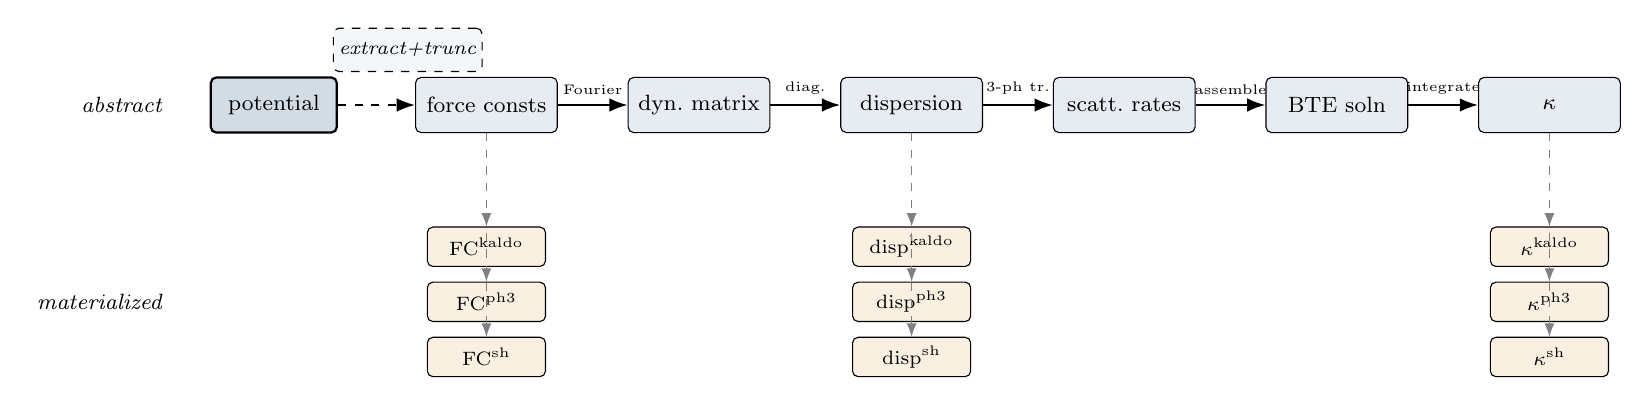
\begin{tikzpicture}[
  >=Latex,
  abstractnode/.style={draw, rounded corners=2pt, minimum width=1.8cm, minimum height=0.7cm,
                       font=\footnotesize, fill=abstrcol!12, inner sep=2pt},
  rootnode/.style={draw, rounded corners=2pt, minimum width=1.6cm, minimum height=0.7cm,
                   font=\footnotesize, fill=abstrcol!22, inner sep=2pt, thick},
  stubnode/.style={draw, dashed, rounded corners=2pt, minimum width=1.6cm, minimum height=0.55cm,
                   font=\scriptsize\itshape, fill=abstrcol!5, inner sep=2pt},
  matnode/.style={draw, rounded corners=2pt, minimum width=1.5cm, minimum height=0.5cm,
                  font=\scriptsize, fill=numcol!12, inner sep=1.5pt},
  arr/.style={->, thick},
  stubarr/.style={->, thick, dashed},
  thinarr/.style={->, dashed, gray, thin},
  oplabel/.style={font=\tiny, midway, above},
  rowlabel/.style={font=\footnotesize\itshape, anchor=east},
]

\node[rootnode]     (POT)   at (-2.7,0) {potential};
\node[stubnode]     (STUB)  at (-1.0,0.7) {extract+trunc};
\node[abstractnode] (FC)    at ( 0.0,0) {force consts};
\node[abstractnode] (DM)    at ( 2.7,0) {dyn.\ matrix};
\node[abstractnode] (DISP)  at ( 5.4,0) {dispersion};
\node[abstractnode] (SR)    at ( 8.1,0) {scatt.\ rates};
\node[abstractnode] (BTE)   at (10.8,0) {BTE soln};
\node[abstractnode] (KAPPA) at (13.5,0) {$\kappa$};

\draw[stubarr] (POT)  -- (FC);
\draw[arr] (FC)   -- node[oplabel] {Fourier}   (DM);
\draw[arr] (DM)   -- node[oplabel] {diag.}     (DISP);
\draw[arr] (DISP) -- node[oplabel] {3-ph tr.}  (SR);
\draw[arr] (SR)   -- node[oplabel] {assemble}  (BTE);
\draw[arr] (BTE)  -- node[oplabel] {integrate} (KAPPA);

\node[rowlabel] at (-4.0,0) {abstract};

\foreach \name/\xpos/\labelk/\labelp/\labels in {
  FCm/0.0/{FC$^{\text{kaldo}}$}/{FC$^{\text{ph3}}$}/{FC$^{\text{sh}}$},
  Dm/5.4/{disp$^{\text{kaldo}}$}/{disp$^{\text{ph3}}$}/{disp$^{\text{sh}}$},
  Km/13.5/{$\kappa^{\text{kaldo}}$}/{$\kappa^{\text{ph3}}$}/{$\kappa^{\text{sh}}$}
}{
  \node[matnode] (\name K) at (\xpos,-1.8) {\labelk};
  \node[matnode] (\name P) at (\xpos,-2.5) {\labelp};
  \node[matnode] (\name S) at (\xpos,-3.2) {\labels};
}

\node[rowlabel] at (-4.0,-2.5) {materialized};

\foreach \src/\dst in {FC/FCmK, FC/FCmP, FC/FCmS,
                       DISP/DmK, DISP/DmP, DISP/DmS,
                       KAPPA/KmK, KAPPA/KmP, KAPPA/KmS}{
  \draw[thinarr] (\src.south) -- (\dst.north);
}

\end{tikzpicture}%
}
\caption{Abstract DAG for lattice thermal conductivity (top, blue) and three of its
materializations (bottom, orange) at selected canonical states (force constants, dispersion,
$\kappa$). The DAG is rooted at the abstract \texttt{Potential}; the dashed
\textit{extract+trunc} edge to \texttt{ForceConstants} represents the upstream operations
(extraction of the $n$-th derivative of $V$ and truncation of the Taylor expansion at order $n$),
which are declared in the substrate but stubbed in Phase 1. Each abstract state has up to one
materialization per code (kaldo, phono3py, ShengBTE); intermediate states between the three
shown follow the same pattern. Discretization choices and code-specific operations live in the
materialized graphs but not in the abstract one. Cross-code reconciliation reduces to comparing
materializations sharing a common abstract parent.}
\label{fig:dag}
\end{figure}

\subsection{The three materialization functors}

Each of the three codes defines a materialization functor:

\begin{itemize}[leftmargin=2em]
  \item \textbf{kaldo} (Python). Computes harmonic and anharmonic phonon transport from
        force constants, supporting iterative BTE, RTA, and the Wigner formulation. Most
        intermediate states are exposed via Python attributes on the \texttt{Phonons} object.
  \item \textbf{phono3py} (C/Python). Computes lattice thermal conductivity from third-order
        force constants, with extensive support for finite-displacement and DFPT pipelines.
        Intermediate quantities are exposed in HDF5 outputs.
  \item \textbf{ShengBTE} (Fortran/MPI). Solves the full linearized BTE with iterative
        self-consistency, exposing intermediate quantities in plain-text output files.
\end{itemize}

For each code, a thin adapter reads the code's natural output (Python attribute, HDF5 dataset, or
text file), constructs the corresponding materialization, and tags it with the abstract state it
realizes. The first concrete demonstrable result of the substrate is to run all three codes on a
single material (silicon) at a single discretization, and to display the three materialized DAGs
aligned to the shared abstract template.

\subsection{Phase 1 scientific capabilities}

Phase 1 yields two immediate scientific capabilities, each of which is an artifact the field does
not currently produce. A third capability is the long-term goal toward which the substrate is
oriented but is deferred to Phase 2.

\begin{itemize}[leftmargin=2em]
  \item \textbf{Cross-code reconciliation at canonical intermediate states.} When kaldo and
        ShengBTE disagree on a final $\kappa$, the substrate localizes the divergence to the
        first abstract state at which the materializations stop agreeing, and attributes it to a
        specific operation along the provenance. This is a structural diagnosis: the substrate
        identifies where two codes do something different, regardless of the magnitude of the
        difference.
  \item \textbf{A unified framework for theory-experiment comparison.} The same abstract DAG
        accepts experimental measurements as additional materializations of parameter states,
        with the same alignment machinery as for cross-code comparison. Phase 1 demonstrates the
        framework on at least one experimental dataset (e.g., a measured $\kappa(T)$ curve for
        silicon).
\end{itemize}

\noindent\textbf{Deferred to Phase 2:}
\begin{itemize}[leftmargin=2em]
  \item \textbf{Decomposed error bounds on $\kappa$.} The substrate is designed to eventually
        produce the central value of $\kappa$ together with a symbolic decomposition of its
        total error into the truncation error of the perturbation series and the discretization
        error of the chosen mesh. The architecture supports this; the implementation of the
        composition algebra is a research problem reserved for Phase 2.
\end{itemize}

\section{Open Questions and Deferred Decisions}
\label{sec:open}

We list the architectural questions that remain open and the principled grounds on which they
were deferred.

\subsection{Algebra of error composition (deferred to Phase 2)}

The substrate is designed to carry error formulas as symbolic expressions, but Phase 1 does not
implement the algebra by which they compose. Composing two errors in independent small parameters
($O(\lambda^4) + O(N^{-2})$) is well-defined; composing two errors in the same parameter requires
care; composing constant-offset errors (e.g., basis-set incompleteness) with asymptotic ones is
yet another case. The right algebra is itself a research subproblem and will be developed
alongside concrete worked examples in Phase 2. The Phase 1 type system reserves the slots
required for error formulas (operation metadata, discretization error model, materialization
total error) but populates them with placeholders rather than computed compositions.

\subsection{When to lift to Lean}

We have committed to keeping the substrate Lean-compatible without being Lean-dependent. The
question of when (and whether) to actually project the abstract layer into Lean is deferred until
the Python prototype has stabilized. A reasonable trigger for this decision is the moment at
which we have enough concrete examples that designing Lean types in isolation becomes
counterproductive.

\subsection{Provenance equivalence}

We have committed to provenance as essential to identity. This means two states with the same
type but different histories are formally distinct. In some cases, however, the two histories are
\emph{equivalent}: they produce identical physics under a theorem we can prove (e.g., Fourier
transform of a real symmetric matrix and direct frequency-domain assembly should yield the same
\texttt{Dispersion}). The substrate must provide a mechanism for declaring such equivalences,
either as explicit axioms or as proven theorems. The mechanism's design is deferred to Day 2
because we want concrete examples before designing the equivalence calculus.

\subsection{Sprint 1 scope}

The first concrete deliverable is a Python implementation. We have considered three scopes:

\begin{enumerate}[leftmargin=2em]
  \item \emph{Narrowest:} kaldo only, harmonic sub-DAG (force constants $\to$ dynamical matrix
        $\to$ dispersion). 4--5 states, fastest to ship.
  \item \emph{Recommended:} kaldo only, full thermal-conductivity DAG. 10--15 states, end-to-end
        on silicon. The substrate skeleton plus one full adapter.
  \item \emph{Broader:} kaldo plus phono3py, full DAG. Validates the cross-code story earlier but
        adds adapter work in parallel with substrate design.
\end{enumerate}

The recommended scope (option 2) is the smallest scope that is still a credible proof of concept
of the substrate, and the choice of one adapter (kaldo) lets us validate the substrate design
before generalizing. Sprint 2 adds phono3py and ShengBTE adapters, at which point the cross-code
demo of \S\ref{sec:demo} becomes real.

\subsection{Implementation language}

We have committed to Python for Sprint 1. The trade-offs were:

\begin{itemize}[leftmargin=2em]
  \item \textbf{Python (chosen).} All target codes have Python bindings or wrappable interfaces.
        The Python type system, augmented with \texttt{pydantic} or \texttt{attrs} and runtime
        checks, is sufficient for the substrate's first-cut type discipline. The development
        speed is dominant, since adapter work is the bulk of the time cost.
  \item \emph{Typed compiled language (Rust, OCaml, TypeScript).} Stronger type guarantees from
        the start. Rejected for Sprint 1 because the foreign-function interface to existing
        Python codes adds friction proportional to the substrate's surface, and we want
        substrate iteration to be cheap.
  \item \emph{Lean.} Considered (\S\ref{ssec:physlean}) and deferred. Not the right tool for
        running scientific computations; reserved as a verification target.
\end{itemize}

\section{Outlook}
\label{sec:outlook}

The substrate is an architectural commitment, not an implementation. The implementation that
follows is scoped to a Python skeleton plus adapters for three thermal-transport codes. The
artifact that motivates the project---a paper-worthy demonstration of cross-code reconciliation
and decomposed error bounds for lattice thermal conductivity---is downstream of the substrate but
is the substrate's first proof-of-value.

Three longer-term directions follow naturally from the design:

\begin{itemize}[leftmargin=2em]
  \item \textbf{Verification.} Project the abstract layer into Lean (via PhysLean or alongside
        it), allowing approximation theorems to be formally proved rather than asserted. The
        provenance mechanism makes this projection well-defined: each operation in $\pi$
        corresponds to a Lean lemma whose statement is the operation's error formula.
  \item \textbf{Theory-experiment integration.} Extend the materialization functor to ingest
        experimental observables. The substrate's graph-alignment machinery applies uniformly,
        so a measured $\kappa$ becomes another materialization of the abstract $\kappa$, and
        ``does the theory match experiment'' becomes graph-alignment with one functor being
        empirical.
  \item \textbf{Grounded LLM agents.} An LLM operating over typed abstract states (rather than
        text tokens) constructs workflows by emitting symbolic operations. The substrate
        type-checks each emission, eliminating the drift problem that plagues current
        text-token agents. The action space is finite, typed, and physically meaningful.
\end{itemize}

The unifying claim of the design is that scientific computing has been organized around the
wrong atomic unit. The instruction-in-an-input-file unit is too low; the natural-language
description is too high; the equation-in-a-paper unit is too disconnected from execution. The
right unit, at least for materials science, is the symbolic operation between typed physics
states. Once that commitment is made, much of the rest of the architecture writes itself.

\bigskip
\hrule
\bigskip

\noindent\emph{This document records the architectural state of the openmaterials-ai project as
of \today. It is intended as the working reference for the project; subsequent revisions should
update the relevant sections rather than appending changelogs.}

\end{document}
